% Документ принадлежит классу article
%\documentclass[a5paper,8pt]{article} 

% Документ принадлежит классу article, боковые отступы для двустраничной печати.
 \documentclass[twoside,a5paper,8pt]{article}

% нормальный юникод и русский язык
\usepackage{cmap}
\usepackage[T2A]{fontenc}
\usepackage[utf8]{inputenc} 
\usepackage[russian,english]{babel} % Пакет поддержки русского языка
% \usepackage[unicode,dvipdfm]{hyperref}
% \usepackage[pdftex,unicode]{hyperref}

% элементы документа
\usepackage{graphicx}
\usepackage{tabularx}
\usepackage{tabulary}
\usepackage{longtable,tabu}

% показывать структуру страницы в виде рамок: поля, отступы и т.п
%\usepackage{showframe}
%\usepackage{fullpage}
\usepackage[margin=15mm]{geometry}

% ширина картинок с изображением деталей
\newlength{\picwidth}
\setlength{\picwidth}{30mm}

% вертикальный отступ между строками таблицы
\renewcommand{\arraystretch}{5}

 \title{Детали набора Робот Машинка, модель 2.1} % Заглавие документа
 \date{\today} % Дата создания

\begin{document}
  \begin{center}
    \textbf{Детали набора Робот Машинка}
  \end{center}
  \begin{flushright}
    \emph{модель 2}
  \end{flushright}
   
  \begin{flushright}
    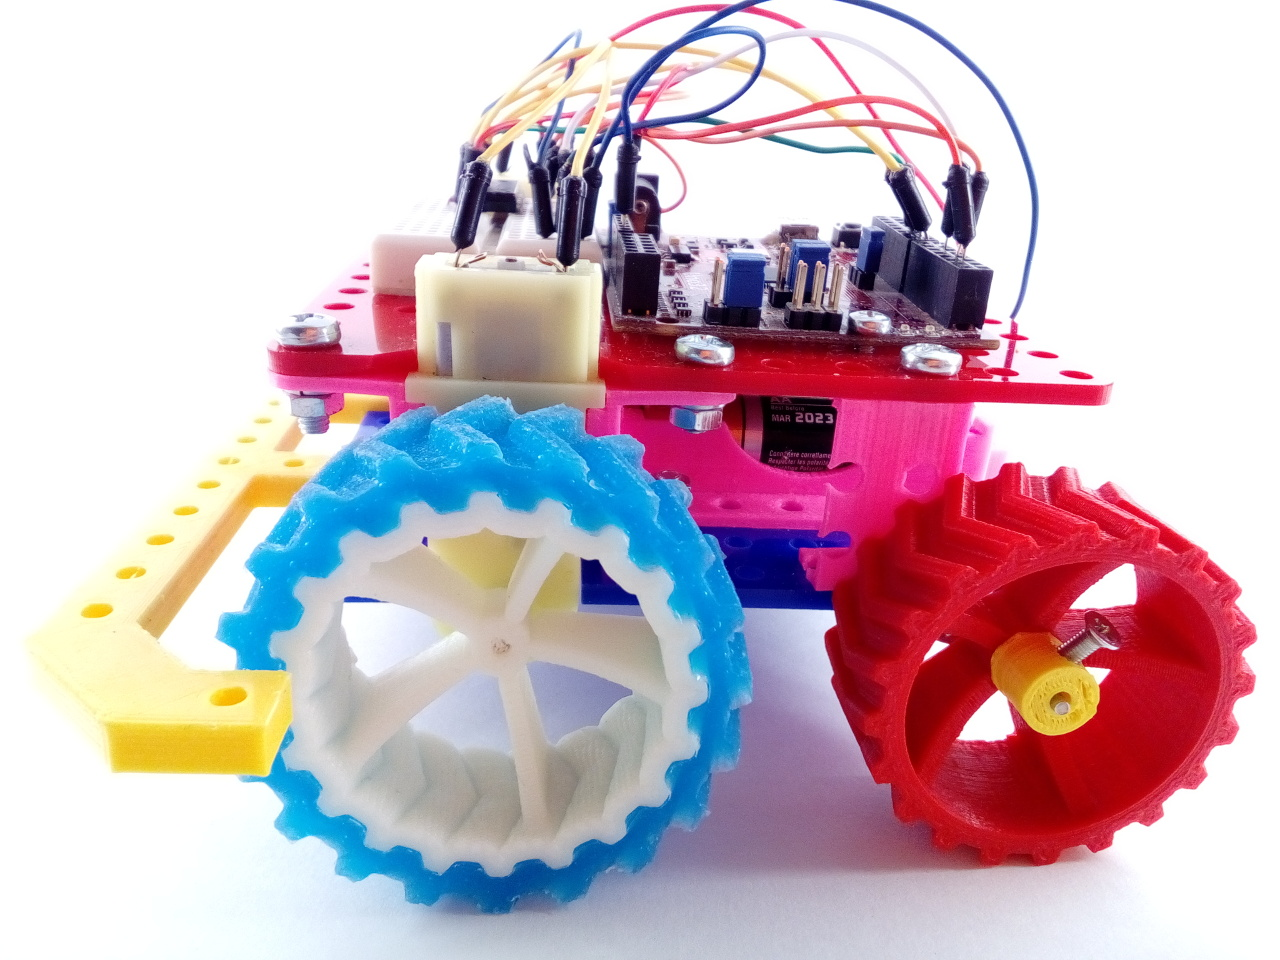
\includegraphics[height=50mm]{fig/robotcar-sideview.jpg}   
  \end{flushright}
  
 % \pagebreak
   
%  \begin{tabularx}{\textwidth}{ X c r }
  \begin{longtabu} to \linewidth { >{\centering}m{45mm}  m{55mm}  m{10mm} }
%  \begin{longtabu} to \linewidth { m{35mm} | p{55mm} | p{10mm} }
% & деталь & количество \\
%  1 & 2 & 3 \\



\includegraphics[width=\picwidth]{fig/wheel-blue.png} & Колёса & 4 шт \\
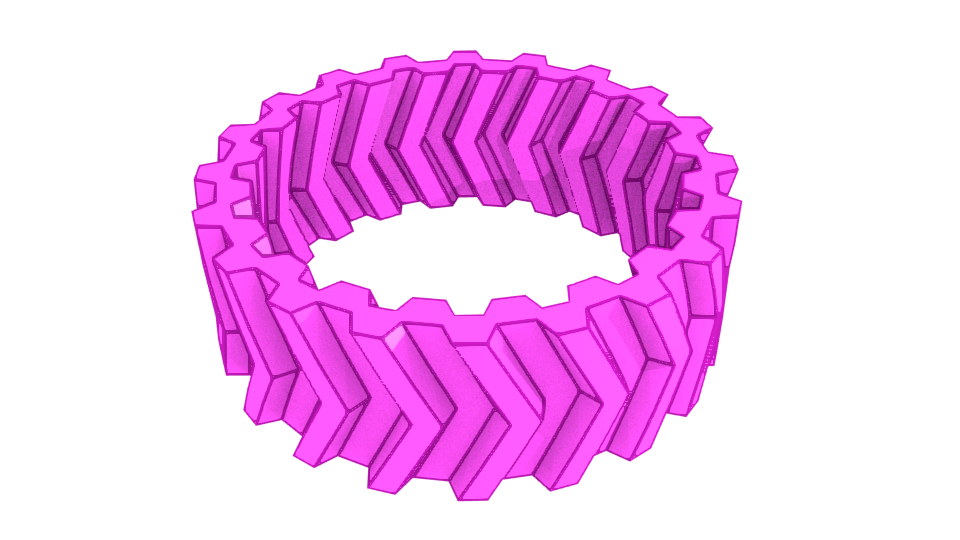
\includegraphics[width=\picwidth]{fig/tyre-pink.png} & Покрышки & 2 шт \\
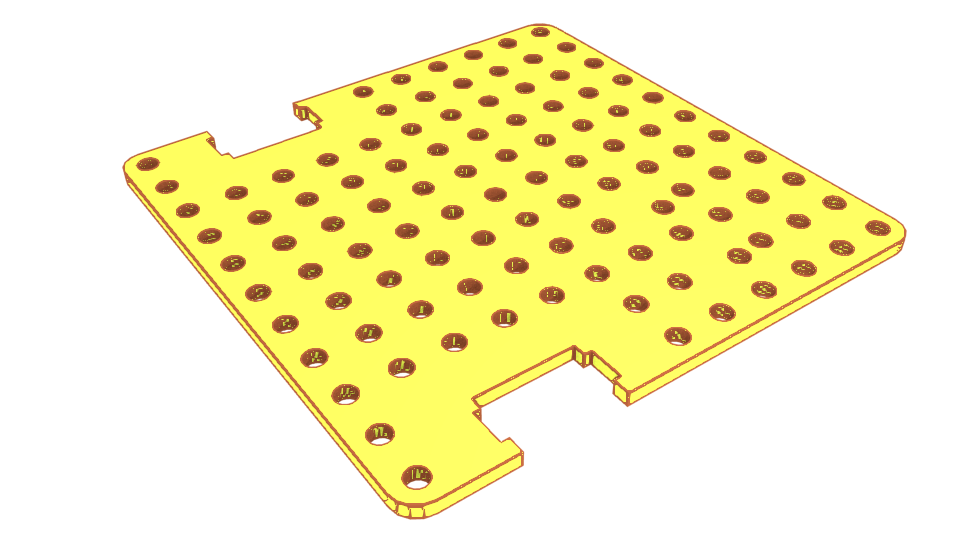
\includegraphics[width=\picwidth]{fig/frame-top-yellow.png} & Верхняя часть корпуса & 1 шт \\
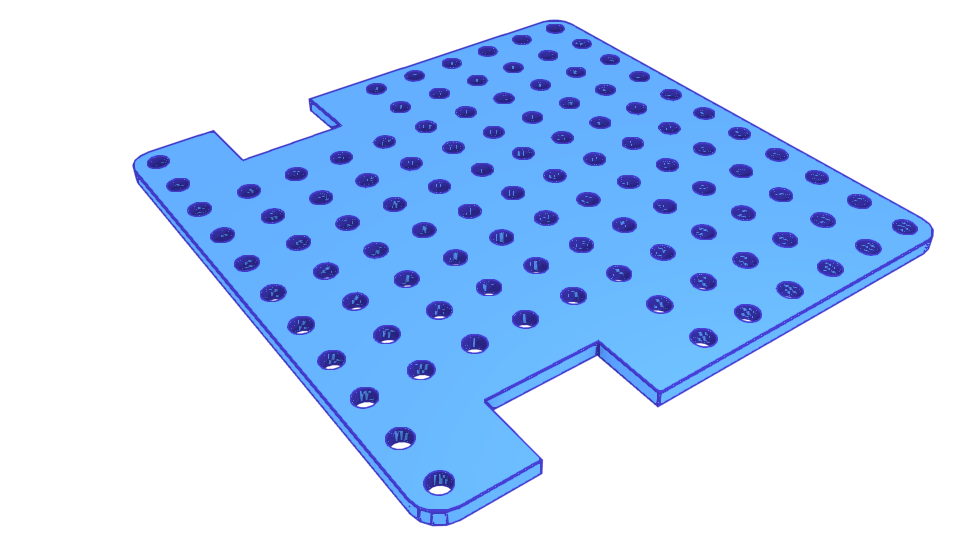
\includegraphics[width=\picwidth]{fig/frame-bottom-blue.png} & Нижняя часть корпуса & 1 шт \\
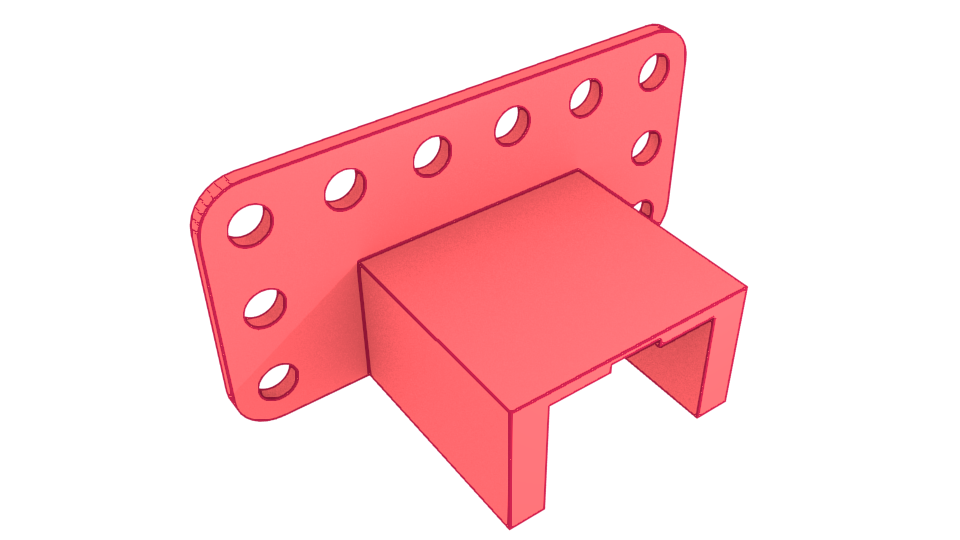
\includegraphics[width=\picwidth]{fig/motor-fix-red.png} & Крепления моторов & 2 шт \\
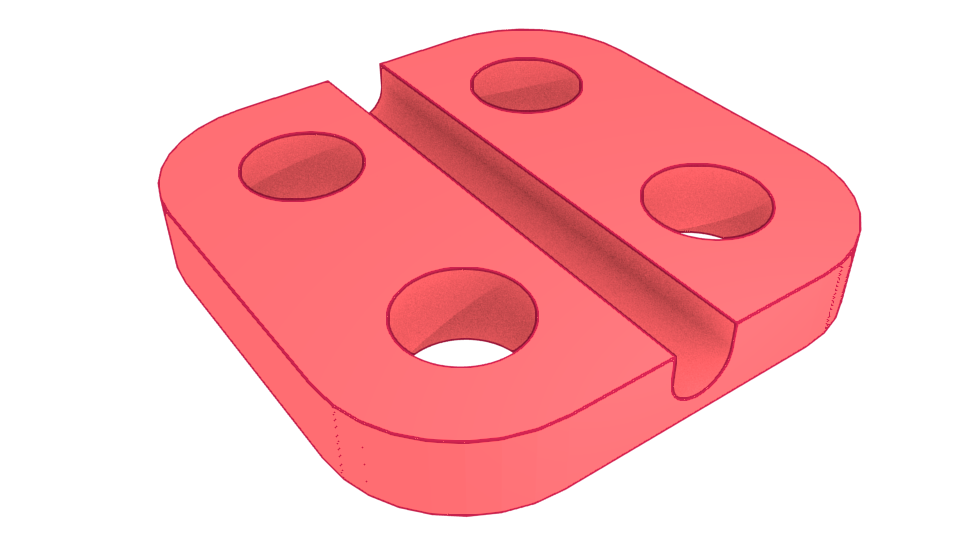
\includegraphics[width=\picwidth]{fig/axis-fix-red.png} & Направляющие для оси & 2 шт \\
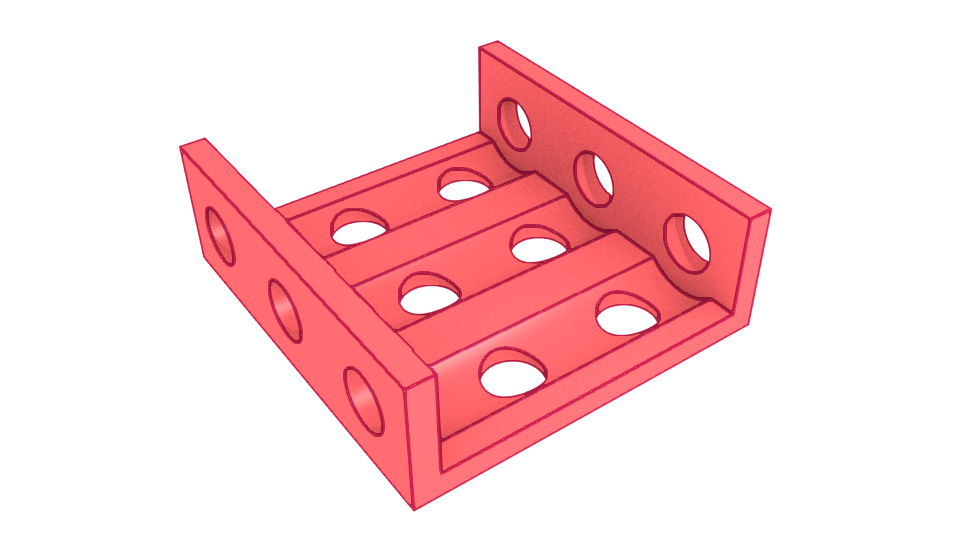
\includegraphics[width=\picwidth]{fig/frame-fix-red.png} & Боковые стенки & 2 шт \\
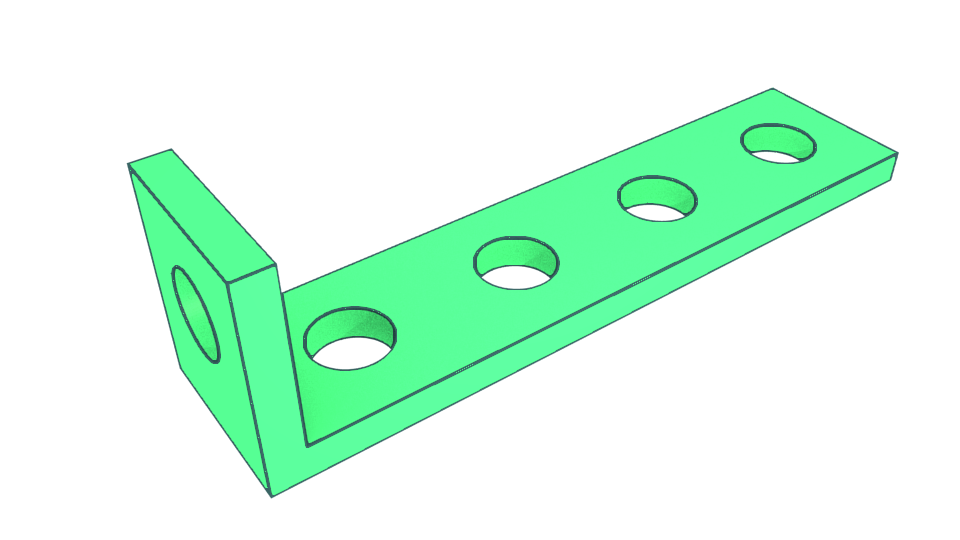
\includegraphics[width=\picwidth]{fig/angle-1x4-green.png} & Уголки & 4 шт \\

\includegraphics[width=\picwidth]{fig/axis-d2mm-l150mm-cherry.png} & Ось для задних колес & 1 шт \\
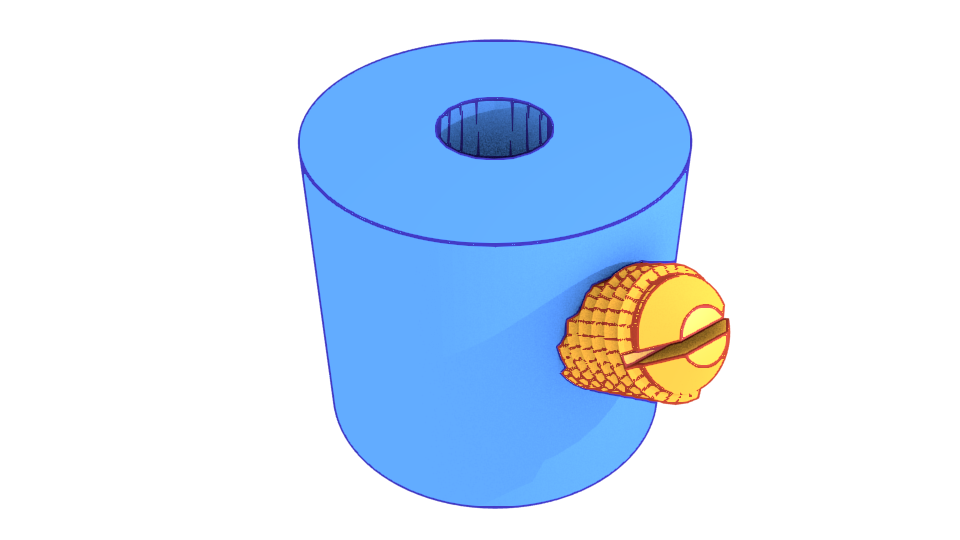
\includegraphics[width=\picwidth]{fig/axis-jam-with-screw-blue.png} & Стопорные втулки на ось & 2 шт \\
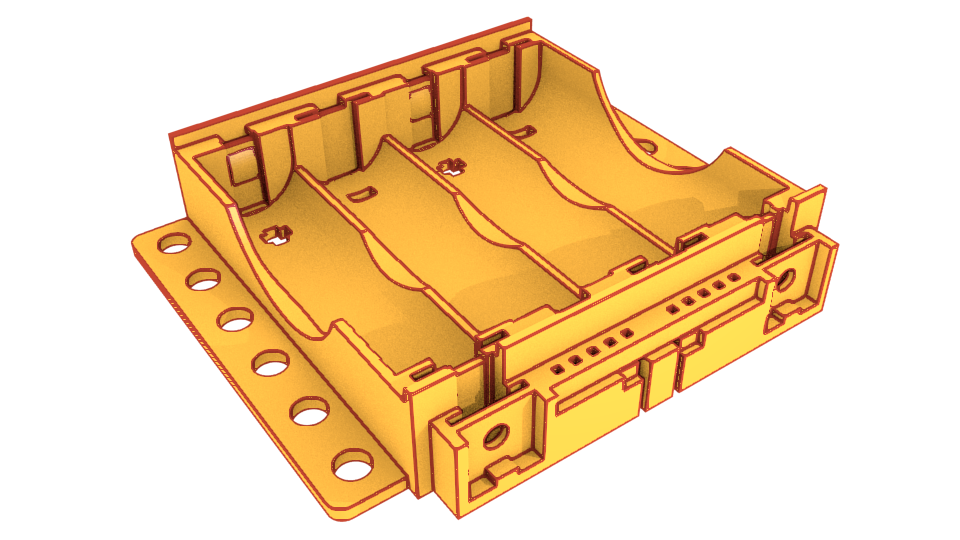
\includegraphics[width=\picwidth]{fig/battery-holder-AAx4-orange.png} & Батарейный отсек 4 АА & 1 шт \\
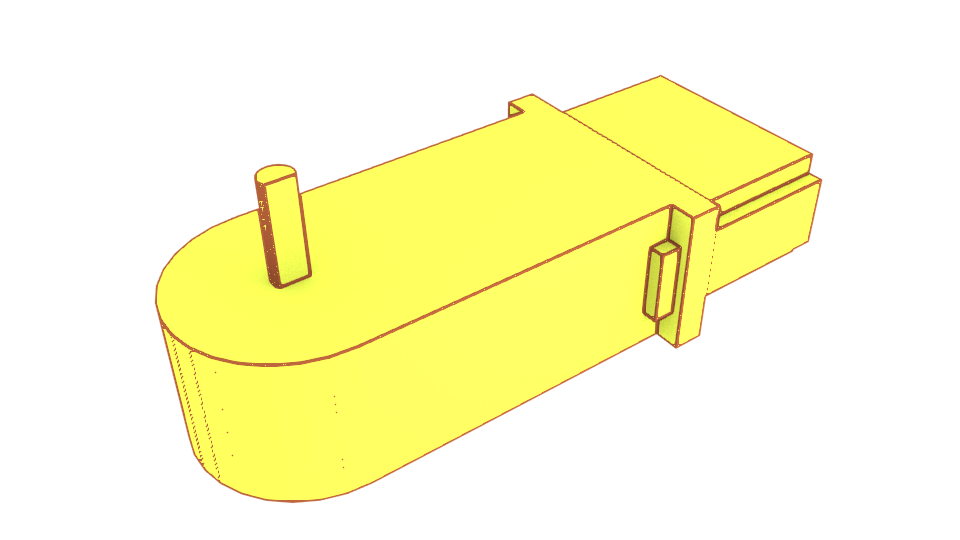
\includegraphics[width=\picwidth]{fig/motor-pololu-yellow.png} & Мотор-редуктор Pololu & 2 шт  \\
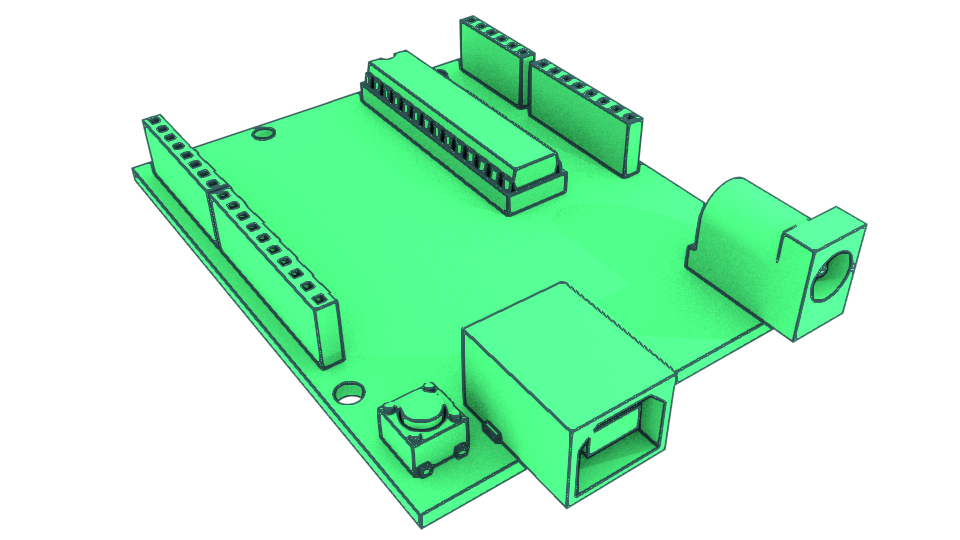
\includegraphics[width=\picwidth]{fig/arduino-uno-green.png} & Плата Arduino Uno & 1 шт \\
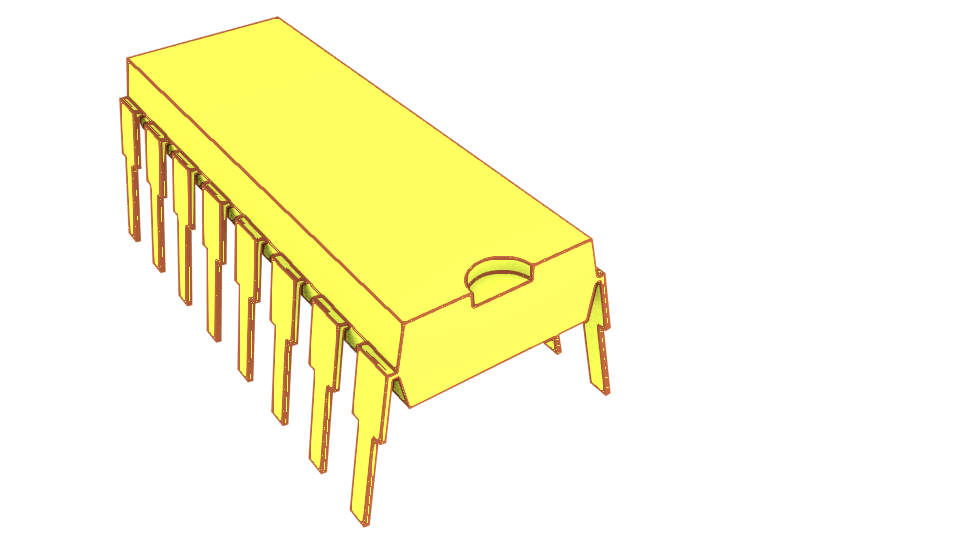
\includegraphics[width=\picwidth]{fig/chip-dip-2x8-yellow.png} & Микросхема L293D (или аналог) & 1 шт \\
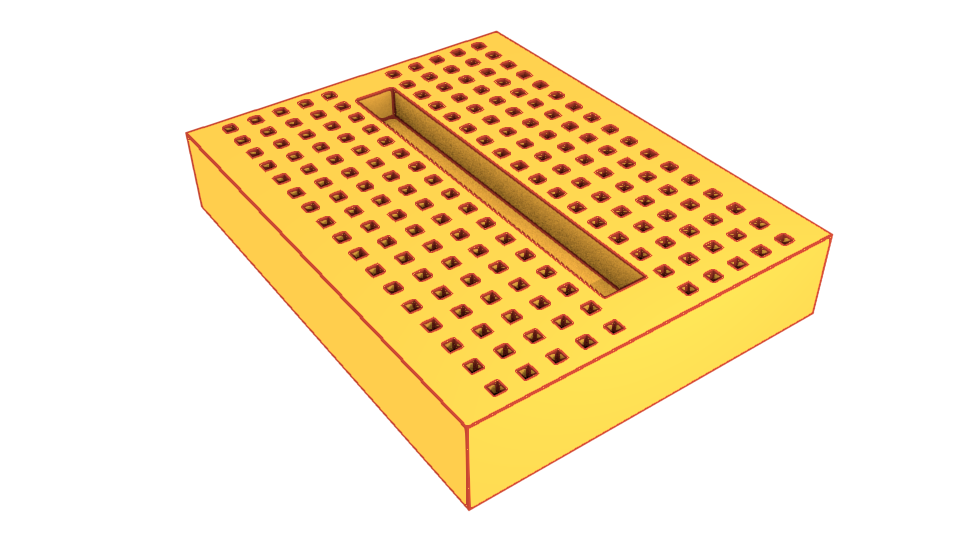
\includegraphics[width=\picwidth]{fig/breadboard-17x10-orange.png} & Макетная плата 17х10 гнезд & 1 шт \\
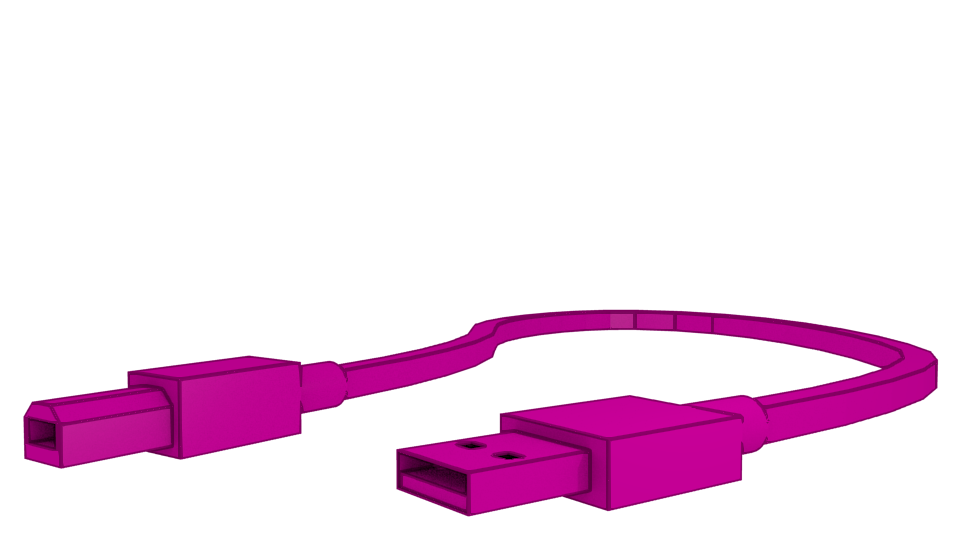
\includegraphics[width=\picwidth]{fig/cable-usb-a-b-cherry.png} & Кабель USB A-B & 1 шт \\
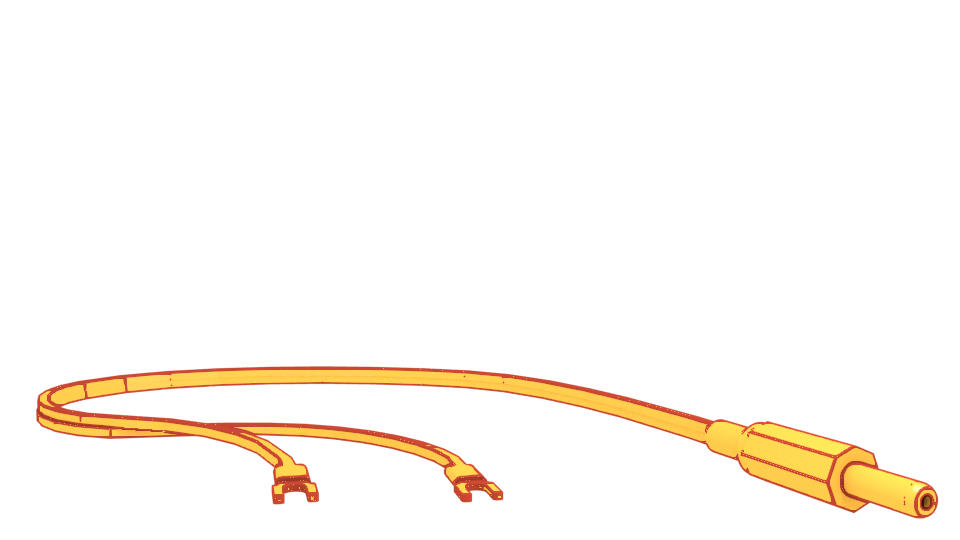
\includegraphics[width=\picwidth]{fig/power-cable-orange.png} & Провод питания платы & 1 шт \\
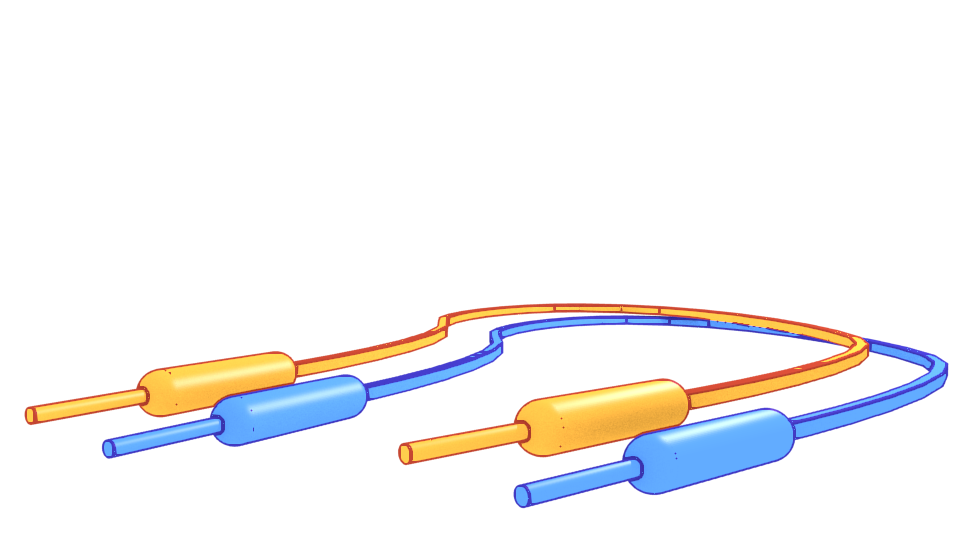
\includegraphics[width=\picwidth]{fig/wire1-1core-pin-pin-2pcs.png} & Набор соединительных проводов & 1 шт \\
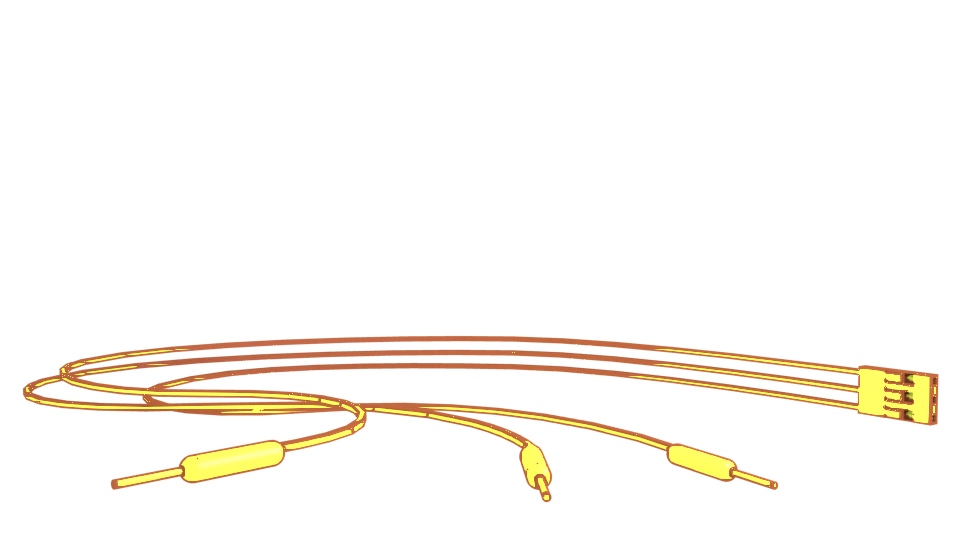
\includegraphics[width=\picwidth]{fig/bus-3pin-female-male-yellow.png} & Шлейф 3 жилы розетка-штепсель & 2 шт \\
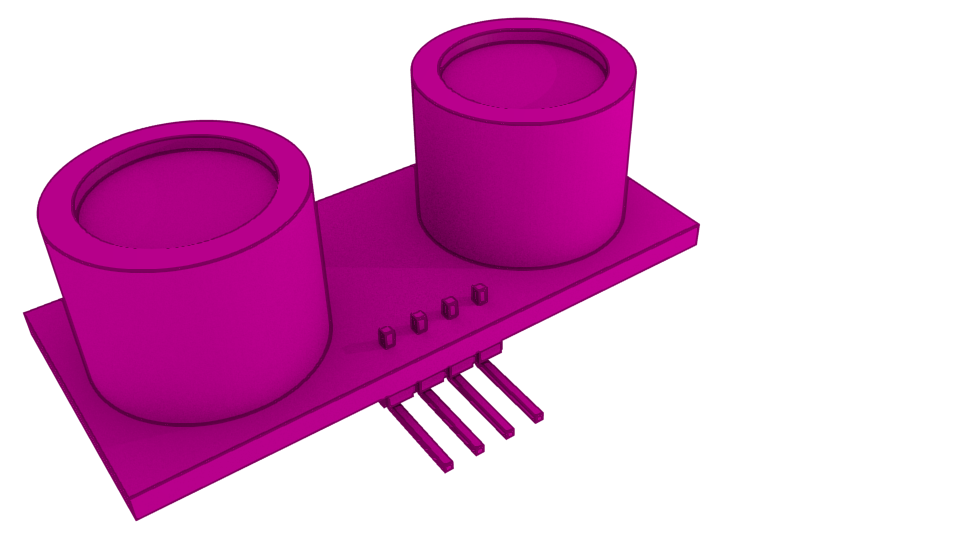
\includegraphics[width=\picwidth]{fig/sonar-cherry.png} & Ультразвуковой дальномер & 1 шт \\
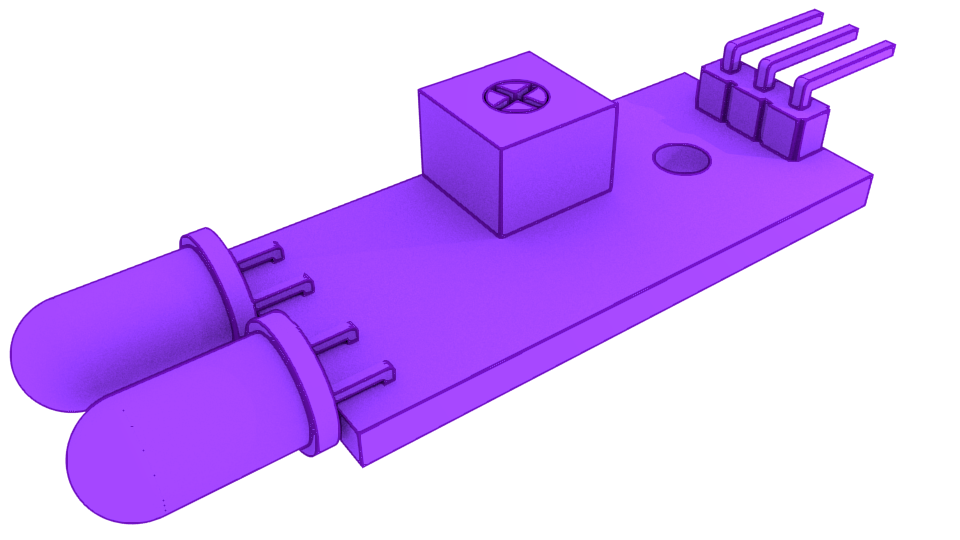
\includegraphics[width=\picwidth]{fig/ir-line-sensor-violete.png} & ИК датчик препятствий & 2 шт \\

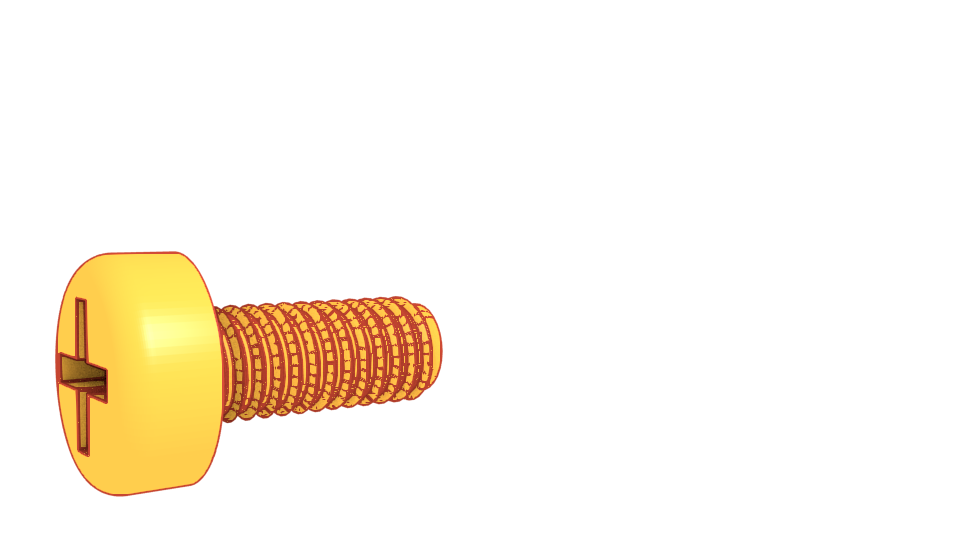
\includegraphics[width=\picwidth]{fig/screws/crosshead-screw-m4x10-orange.png} & Винт M4x10 & 28 шт \\
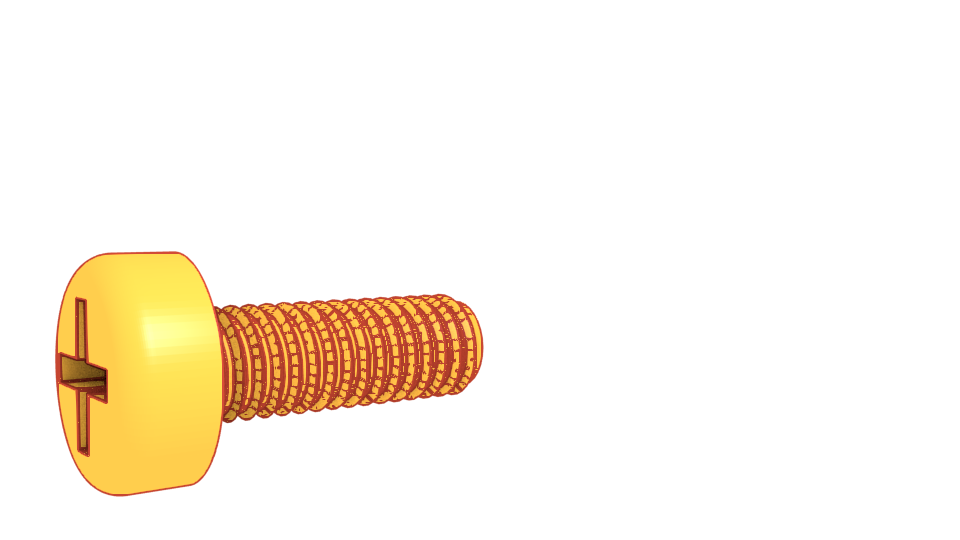
\includegraphics[width=\picwidth]{fig/screws/crosshead-screw-m4x12-orange.png} & Винт M4x12 & 8 шт \\


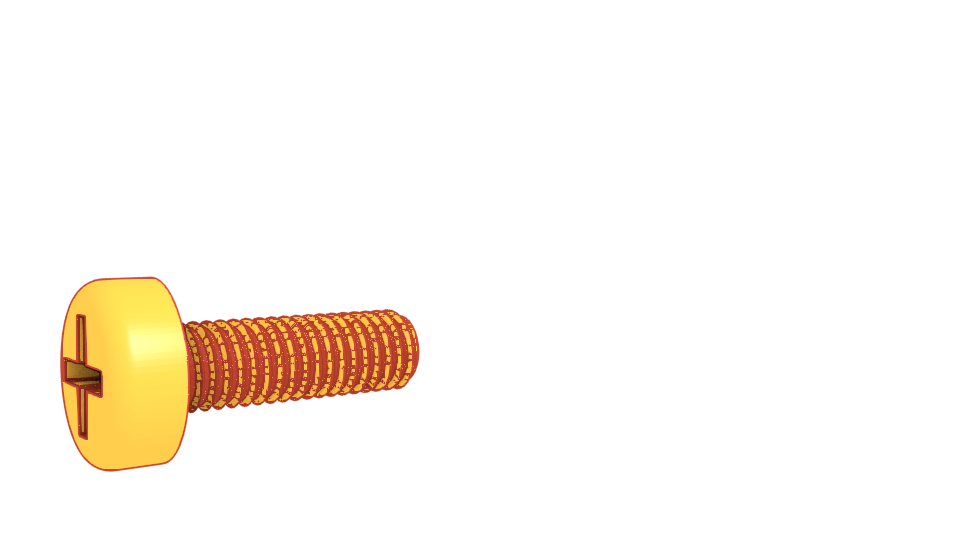
\includegraphics[width=\picwidth]{fig/screws/crosshead-screw-m3x10-orange.png} & Винт M3x10 & 10 шт \\

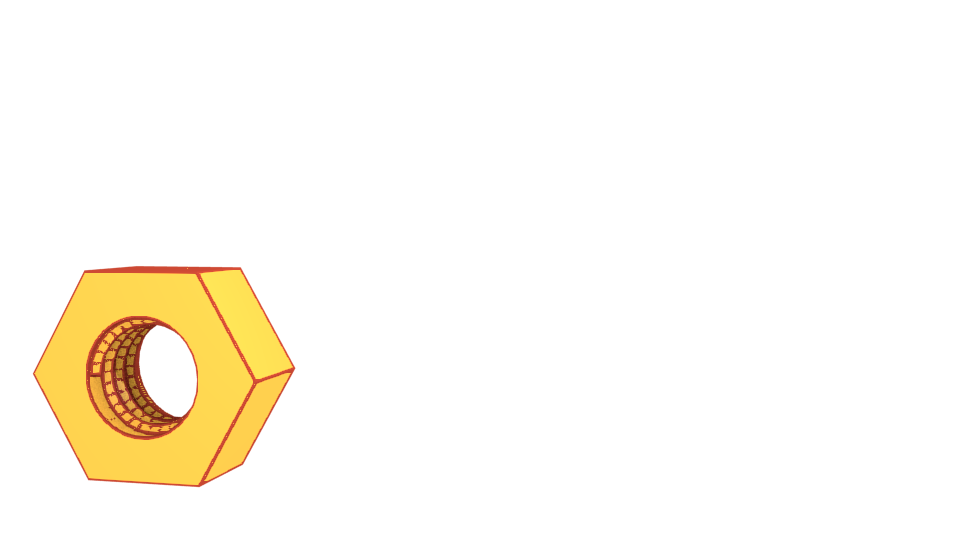
\includegraphics[width=\picwidth]{fig/screws/nut-m4-orange.png} & Гайка M4 & 36 шт \\
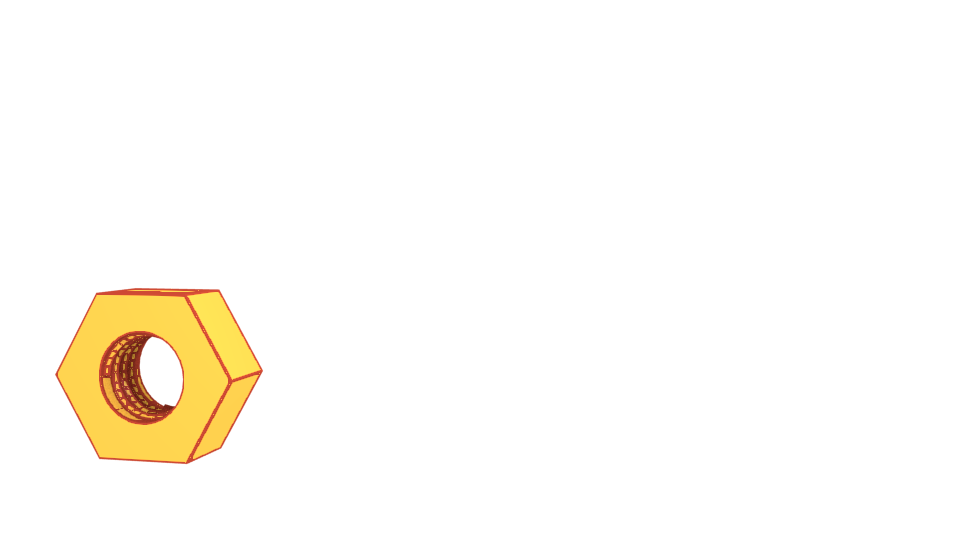
\includegraphics[width=\picwidth]{fig/screws/nut-m3-orange.png} & Гайка M3 & 10 шт \\


\includegraphics[width=\picwidth]{fig/screws/spring-washer-m4-orange.png} & Шайба пружинная M4 & 36 шт \\

\includegraphics[width=\picwidth]{fig/screws/spring-washer-m3-orange.png} & Шайба пружинная M3 & 10 шт \\

  \end{longtabu}   
\end{document}
